\documentclass[iop]{emulateapj}
\bibliographystyle{apj}
\usepackage{graphicx}
\usepackage[suffix=]{epstopdf}
\usepackage{natbib}
\usepackage{amsmath}
\providecommand{\e}[1]{\ensuremath{\times 10^{#1}}}
\usepackage{hyperref}

\submitted{\today}
\journalinfo{}

\shortauthors{Davenport et al.}
\shorttitle{Gender in Astronomy Talks}

\begin{document}


\title{Studying Gender in Conference Talks: Trends from Multiple Conferences}

\author{
	James R. A. Davenport\altaffilmark{1,2}
	}


\altaffiltext{1}{Department of Physics \& Astronomy, Western Washington University, Bellingham, WA 98225}
\altaffiltext{2}{NSF Astronomy and Astrophysics Postdoctoral Fellow}



\begin{abstract}

\end{abstract}



%%%%%%%%%%%%%%%%%%%%%%%%%%%%%%
\section{Introduction}

an ongoing survey, taken up by many people


%%%%%%%%%%%%%%%%%%%%%%%%%%%%%%
\section{Collecting Data}

use same survey form, available on github
https://github.com/jradavenport/gender-web-form


%%%%%%%%%%%%%%%%%%%%%%
\section{Basic Sample Properties}
basic stats for:

AAS 223

AAS 225

CS 16

NAM 2014


%\begin{figure}[!t]
%\centering
%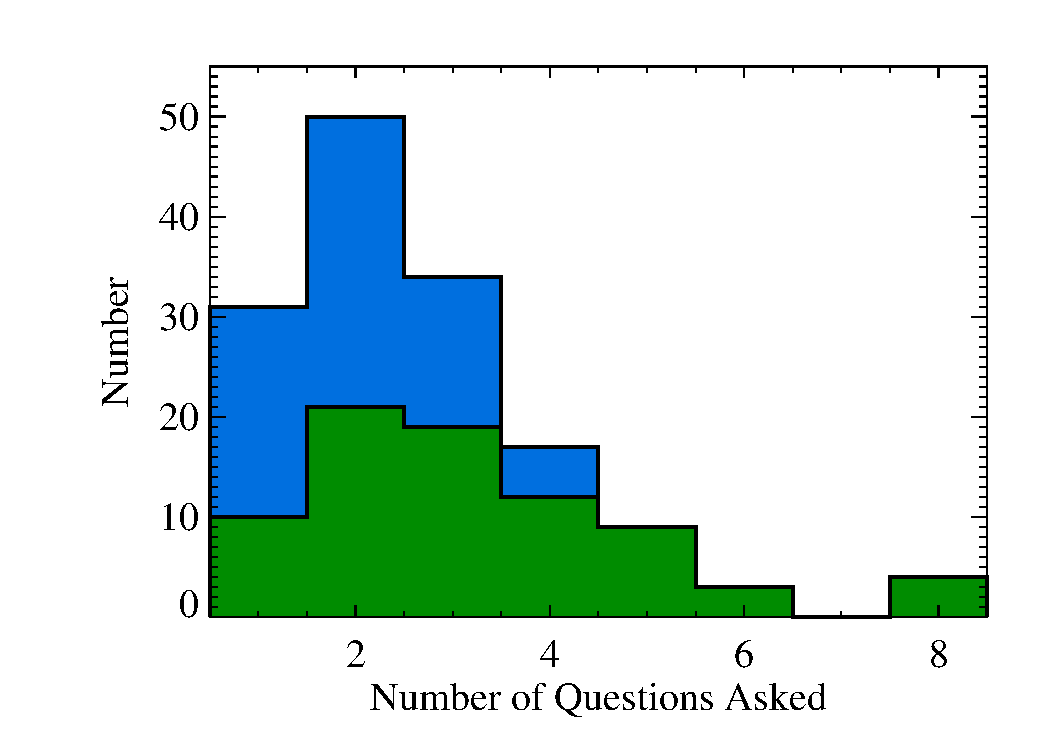
\includegraphics[width=3.5in]{n_question_gender}
%\caption{Number of questions asked per talk as a function of the {\it speaker's} gender.}
%\label{fig:qhist}
%\end{figure}


%%%%%%%%%%%%%%%%%%%%%%%%%%%%%%
\section{Comparing to the Conference Attendees} 
In general, do we see a match?


%%%%%%%%%%%%%%%%%%%%%%%%%%%%%%
\section{Effect of Session Chair Gender}
Do we see this again? Not seen in NAM


%%%%%%%%%%%%%%%%%%%%%%%%%%%%%%
\section{Effect of number of questions}
does Brett's finding hold up?


%%%%%%%%%%%%%%%%%%%%%%%%%%%%%%
\section{Differences between conferences?}


%%%%%%%%%%%%%%%%%%%%%%%%%%%%%%
\section{Differences between subject areas} 
do we dare? i want to!


%%%%%%%%%%%%%%%%%%%%%%%%%%%%%%
\section{Concluding Remarks}

entire data and project is open source
https://github.com/jradavenport/Gender-in-Astro


\acknowledgements
%We graciously thank all the volunteers who helped gather data and provided many useful suggestions throughout the project. Many thanks also to the organizers and sponsors of the AAS 223 Hack Day.




\end{document}
